\section{Instrumenting the Erlang application}
    \subsection{Including the adapter}

    The Erlang project you need to instrument needs to include the adapter in its dependencies, to do that, you need to include it in your dependencies.

    \begin{minted}{text}
        %your_app.app.src
    {application, otel_getting_started, [
        ...
        {applications, [
            kernel,
            stdlib,
            opentelemetry,
            opentelemetry_api,
        opentelemetry_exporter,
        dqsd_otel
        ]},
        ...
        ]}.
    \end{minted}

    \begin{minted}{text}
    {deps, [
    {opentelemetry, "~> 1.3"},
    {opentelemetry_api, "~> 1.2"},
    {opentelemetry_exporter, "~> 1.0"},
    {dqsd_otel, {git, "https://github.com/fnieri/dqsd_otel.git", {tag, "the_latest_version_on_git"}}}
]}.
    \end{minted}
    
    Once you have the dependencies set up you can begin creating outcome instances for the oscilloscope.

    (\textbf{Note:} If the project were to change name, you can still find the project in https://github.com/fnieri/).

    \subsection{Starting spans}
        To start spans you need to call:
        \begin{minted}{erlang}
            {ProbeCtx, Pid} = dqsd_otel:start_span(<<"probe">>, #{attributes => [{attr, <<"my_attr_5o5s10">>}]}),
        \end{minted}
        This will give you the OpenTelemetry context of the probe and the Pid of the process to call upon end. It is left up to you to decide how to carry both in the execution.
        The function calls OpenTelemetry \texttt{?start\_span} macro, effectively replacing it.

    \subsection{Ending spans}
        To end spans you need to call:
        \begin{minted}{erlang}
            dqsd_otel:end_span(ProbeCtx, ProbePid)
        \end{minted}
        This will end the span on the OpenTelemetry side and end the outcome instance if it hasn't timed out.
        The function calls OpenTelemetry \texttt{?end\_span} macro, effectively replacing it.

    \subsection{Failing outcome instances}
        To fail \textbf{custom} spans you need to call:
        \begin{minted}{erlang}
            dqsd_otel:fail_span(WorkerPid),
        \end{minted}
        Contrary to the other methods, this does not end OpenTelemetry spans, it is let up to you to decide how to handle failure in spans.

\section{Establishing the adapter - oscilloscope connection}
    To connect to the oscilloscope to the server, you first need to start the oscilloscope server by setting the oscilloscope listening IP and port on the dashboard.

    \begin{figure}[H]
        \begin{center}
        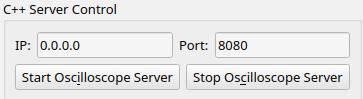
\includegraphics[width = 0.8\textwidth]{img/manual/cserv.png}
        \end{center}
    \end{figure}

    If the server cannot start, a popup will appear with the error.
    
    Once this is done, the adapter can establish a connection to the oscilloscope to send spans. The adapter can now connect to the oscilloscope server. 
    
    \begin{figure}[H]
        \begin{center}
        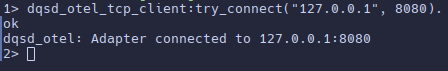
\includegraphics[width = 0.8 \textwidth]{img/manual/connectadapter.png}
        \end{center}
    \end{figure}
    
    We now need to start the listener on the adapter.

     \begin{figure}[H]
        \begin{center}
        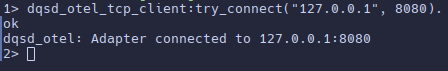
\includegraphics[width = 0.8 \textwidth]{img/manual/connectadapter.png}
        \end{center}
    \end{figure}

    If an error may arrive during the start-up of the listener, it will be printed out.

    Now, we can connect the oscilloscope to the adapter by setting the listener endpoint.
    
     \begin{figure}[H]
        \begin{center}
        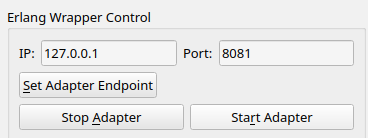
\includegraphics[width = 0.8 \textwidth]{img/manual/endpoint.png}
        \end{center}
    \end{figure}

    If the server cannot connect, an error will popup. Once connected, the server can start and stop the adapter sending of the spans by clicking the two buttons below.
